\documentclass{article}

\usepackage{booktabs} % For \midrule in parameter tables
\usepackage{fullpage} % Set all margins to 1 inch
\usepackage{graphicx}
\usepackage[bookmarksopen=true]{hyperref} % Create section bookmarks
\usepackage{longtable} % Break tables across pages
\usepackage{standalone} % Skips extra preambles in inputted files
\usepackage{tabularx} % Force table to page width
\usepackage{url} % For \path command

\title{Estimation and Forecasting Results. \\ New York Fed DSGE Model m1010, ss20. Model1009, with trend and stationary components in the safety and liquidity premia processes.}
\author{User}

\begin{document}
\maketitle


\section{Specification}

\subsection{User}

\begin{itemize}
  \item Packet creator: matyasfarkas
  \item Creation time: September 5, 2025 at 16:40
\end{itemize}

\subsection{Model}

\begin{itemize}
  \item Model: m1010
  \item Subspec: ss20
  \item Number of states: 91
  \item Number of shocks: 29
  \item Number of observables: 20
  \item Number of parameters: 108
  \item Number of anticipated shocks: 6
\end{itemize}

\subsection{Data}

\begin{itemize}
  \item Input data directory: \path{c:/Mac/Home/Documents/GitHub/rstarBrookings2017/dsge/input_data}
  \item Output data directory: \path{c:/Mac/Home/Documents/GitHub/rstarBrookings2017/dsge}
  \item Data vintage: 250826
  \item Dataset ID: 4
  \item Conditional data vintage: 250905
  \item Conditional dataset ID: 2
  \item Use population forecast: false
  \item Last quarter of data: 2024-Q3
  \item Last quarter of conditional data: 2024-Q4
\end{itemize}


\clearpage
\section{Estimation}

\subsection{Histograms}

\begin{longtable}{cc}
\includegraphics[width=0.45\textwidth]{c:/Mac/Home/Documents/GitHub/rstarBrookings2017/dsge/output_data/m1010/ss20/estimate/figures/prior_posterior_alpha_vint=250826.pdf} &
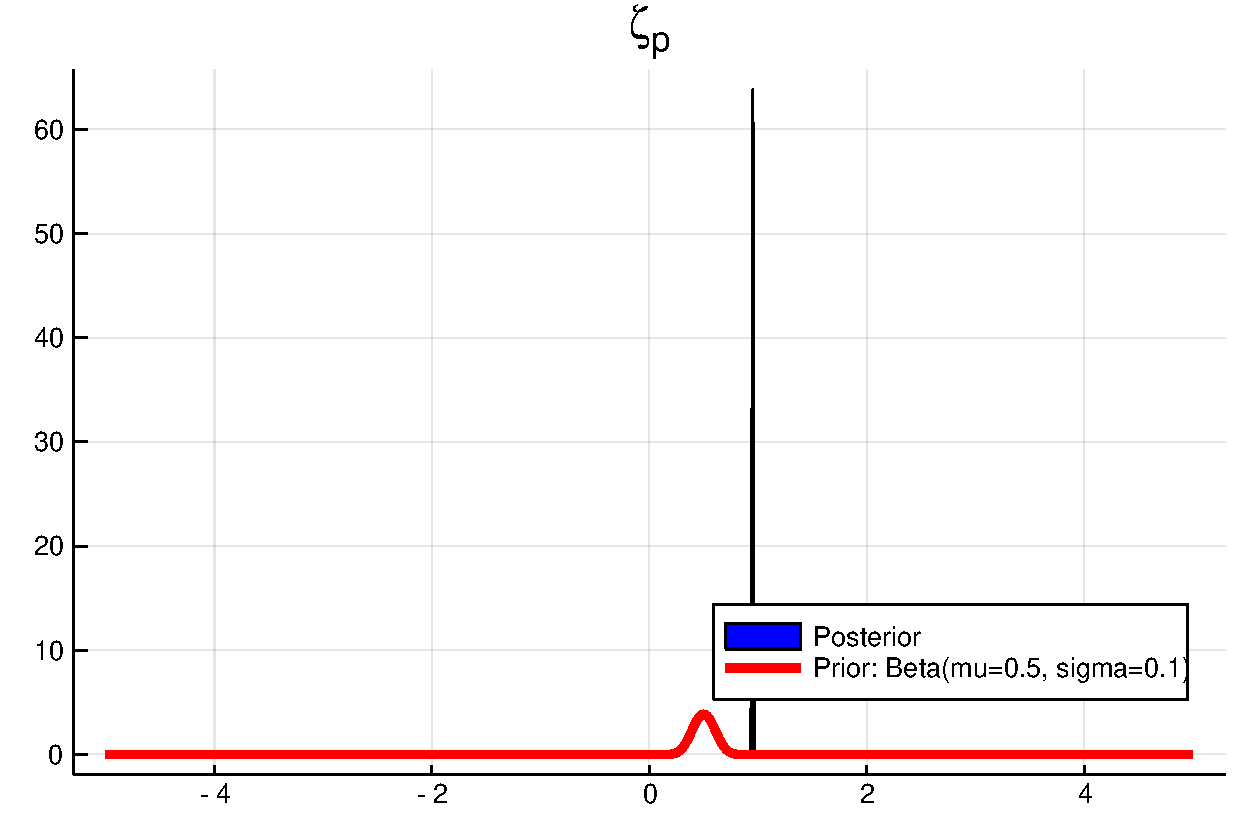
\includegraphics[width=0.45\textwidth]{c:/Mac/Home/Documents/GitHub/rstarBrookings2017/dsge/output_data/m1010/ss20/estimate/figures/prior_posterior_zeta_p_vint=250826.pdf} \\
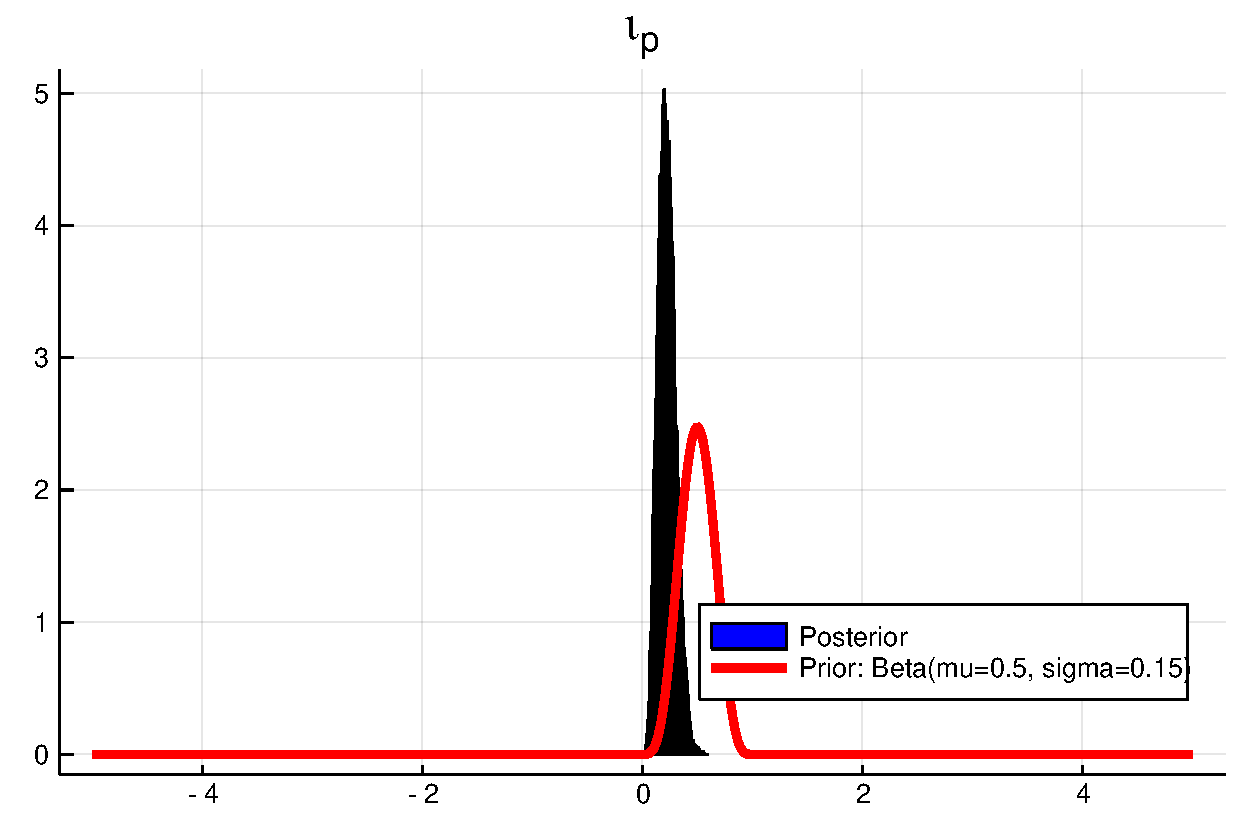
\includegraphics[width=0.45\textwidth]{c:/Mac/Home/Documents/GitHub/rstarBrookings2017/dsge/output_data/m1010/ss20/estimate/figures/prior_posterior_iota_p_vint=250826.pdf} &
\includegraphics[width=0.45\textwidth]{c:/Mac/Home/Documents/GitHub/rstarBrookings2017/dsge/output_data/m1010/ss20/estimate/figures/prior_posterior_S''_vint=250826.pdf} \\
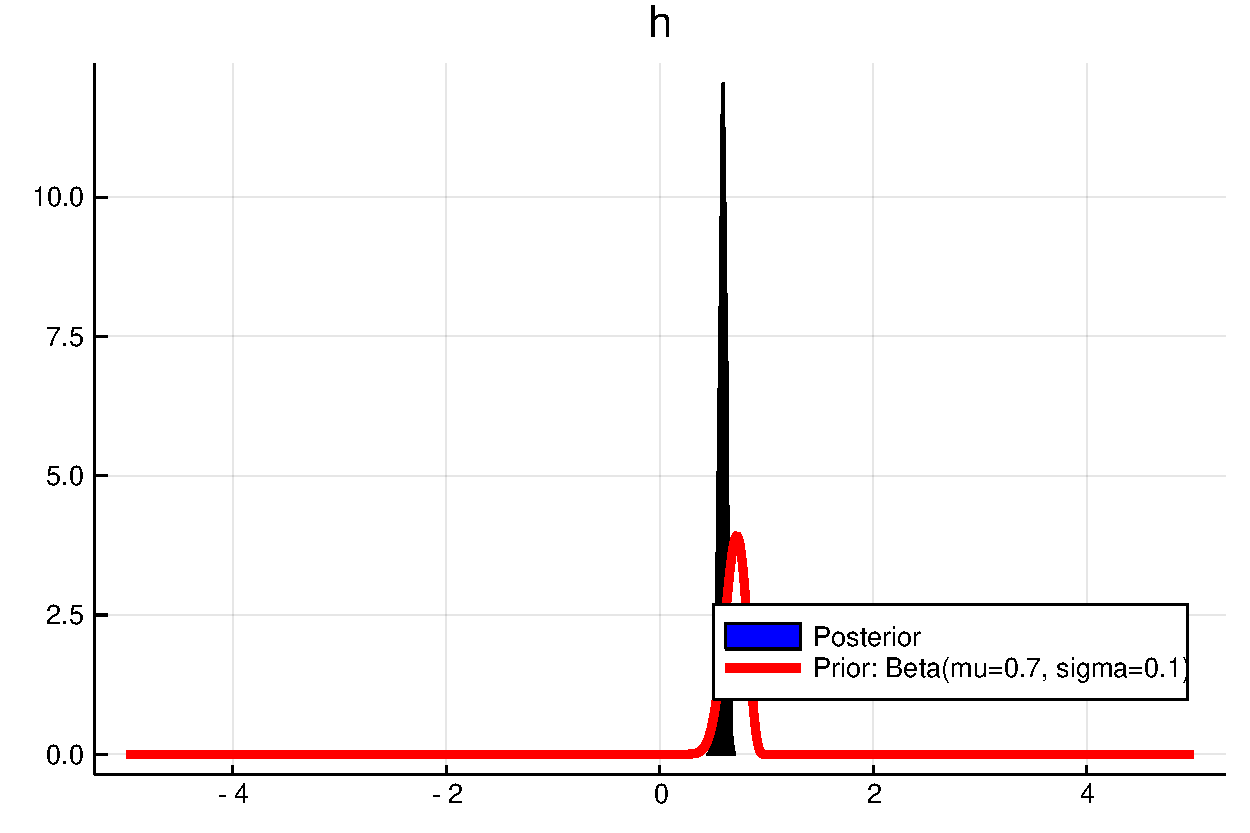
\includegraphics[width=0.45\textwidth]{c:/Mac/Home/Documents/GitHub/rstarBrookings2017/dsge/output_data/m1010/ss20/estimate/figures/prior_posterior_h_vint=250826.pdf} &
\includegraphics[width=0.45\textwidth]{c:/Mac/Home/Documents/GitHub/rstarBrookings2017/dsge/output_data/m1010/ss20/estimate/figures/prior_posterior_ppsi_vint=250826.pdf} \\
\includegraphics[width=0.45\textwidth]{c:/Mac/Home/Documents/GitHub/rstarBrookings2017/dsge/output_data/m1010/ss20/estimate/figures/prior_posterior_nu_l_vint=250826.pdf} &
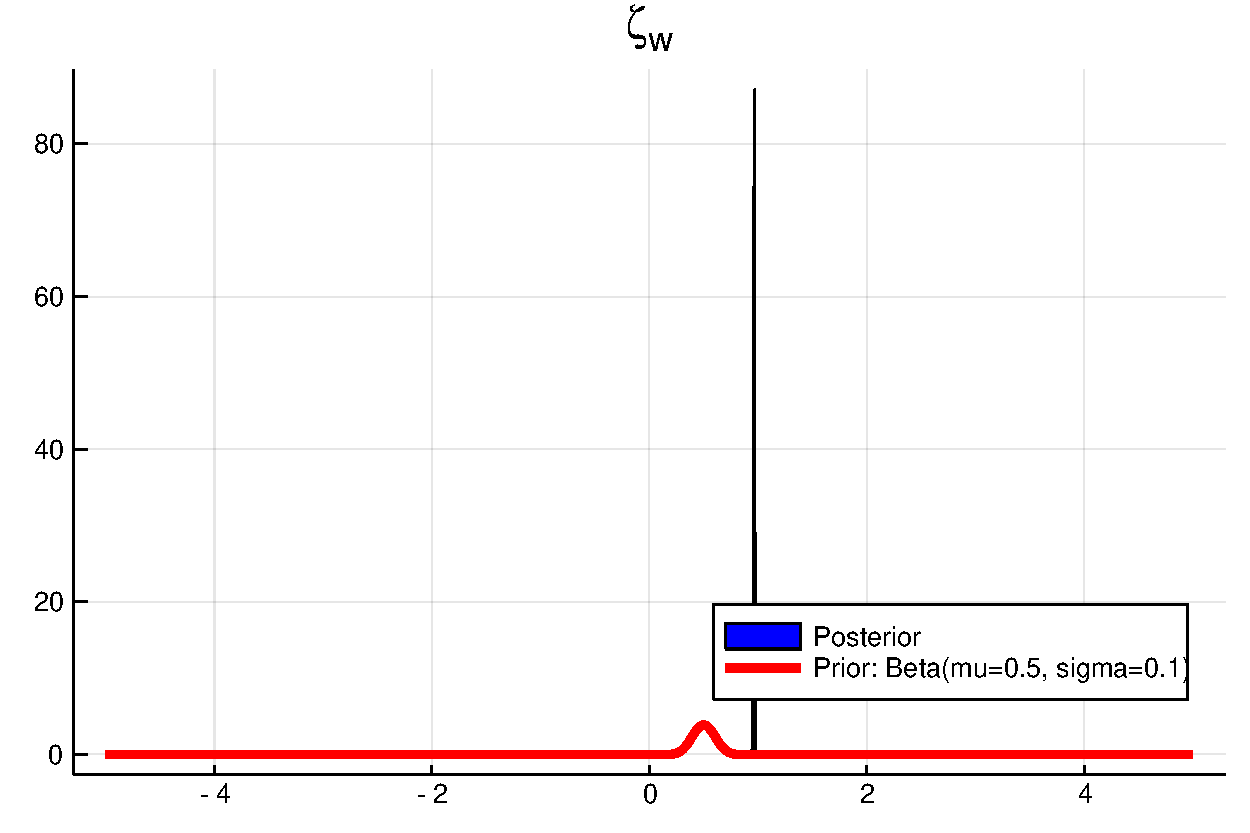
\includegraphics[width=0.45\textwidth]{c:/Mac/Home/Documents/GitHub/rstarBrookings2017/dsge/output_data/m1010/ss20/estimate/figures/prior_posterior_zeta_w_vint=250826.pdf} \\
\includegraphics[width=0.45\textwidth]{c:/Mac/Home/Documents/GitHub/rstarBrookings2017/dsge/output_data/m1010/ss20/estimate/figures/prior_posterior_iota_w_vint=250826.pdf} &
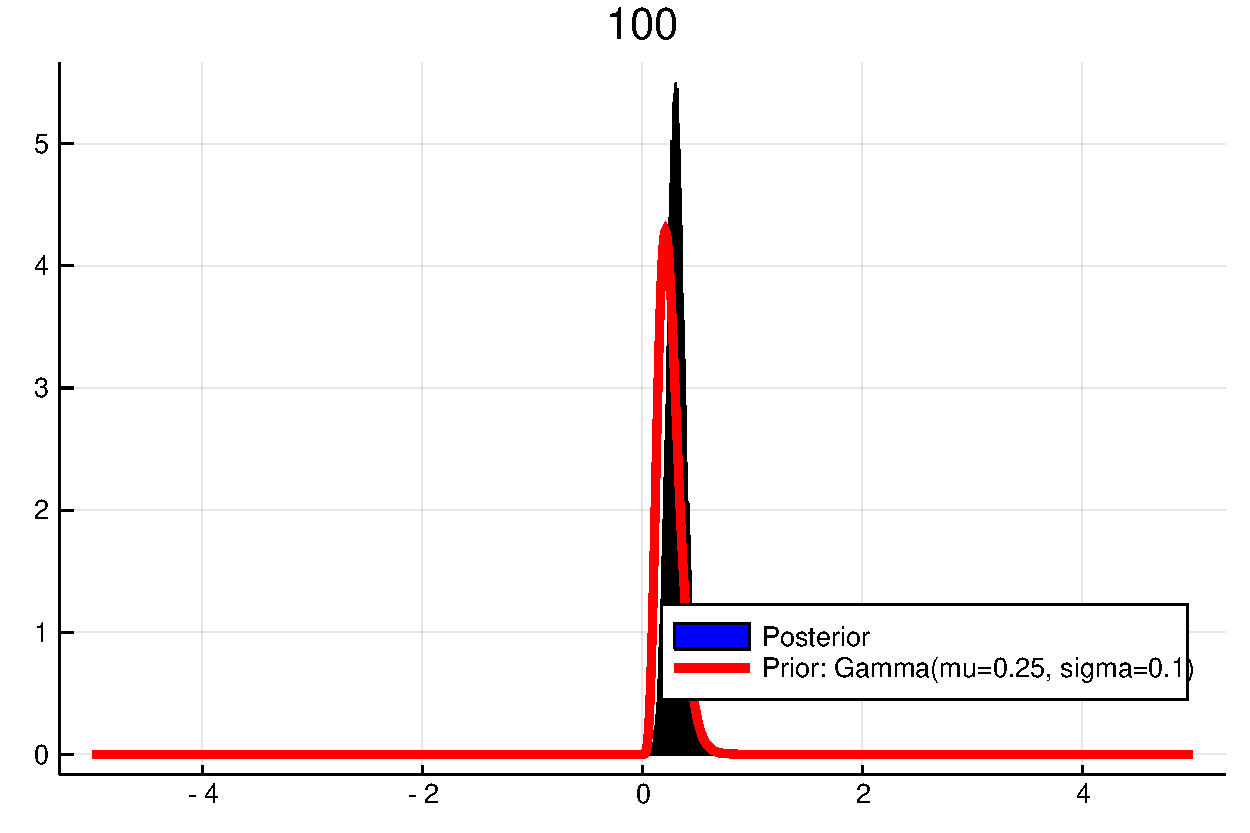
\includegraphics[width=0.45\textwidth]{c:/Mac/Home/Documents/GitHub/rstarBrookings2017/dsge/output_data/m1010/ss20/estimate/figures/prior_posterior_beta_vint=250826.pdf} \\
\includegraphics[width=0.45\textwidth]{c:/Mac/Home/Documents/GitHub/rstarBrookings2017/dsge/output_data/m1010/ss20/estimate/figures/prior_posterior_psi1_vint=250826.pdf} &
\includegraphics[width=0.45\textwidth]{c:/Mac/Home/Documents/GitHub/rstarBrookings2017/dsge/output_data/m1010/ss20/estimate/figures/prior_posterior_psi2_vint=250826.pdf} \\
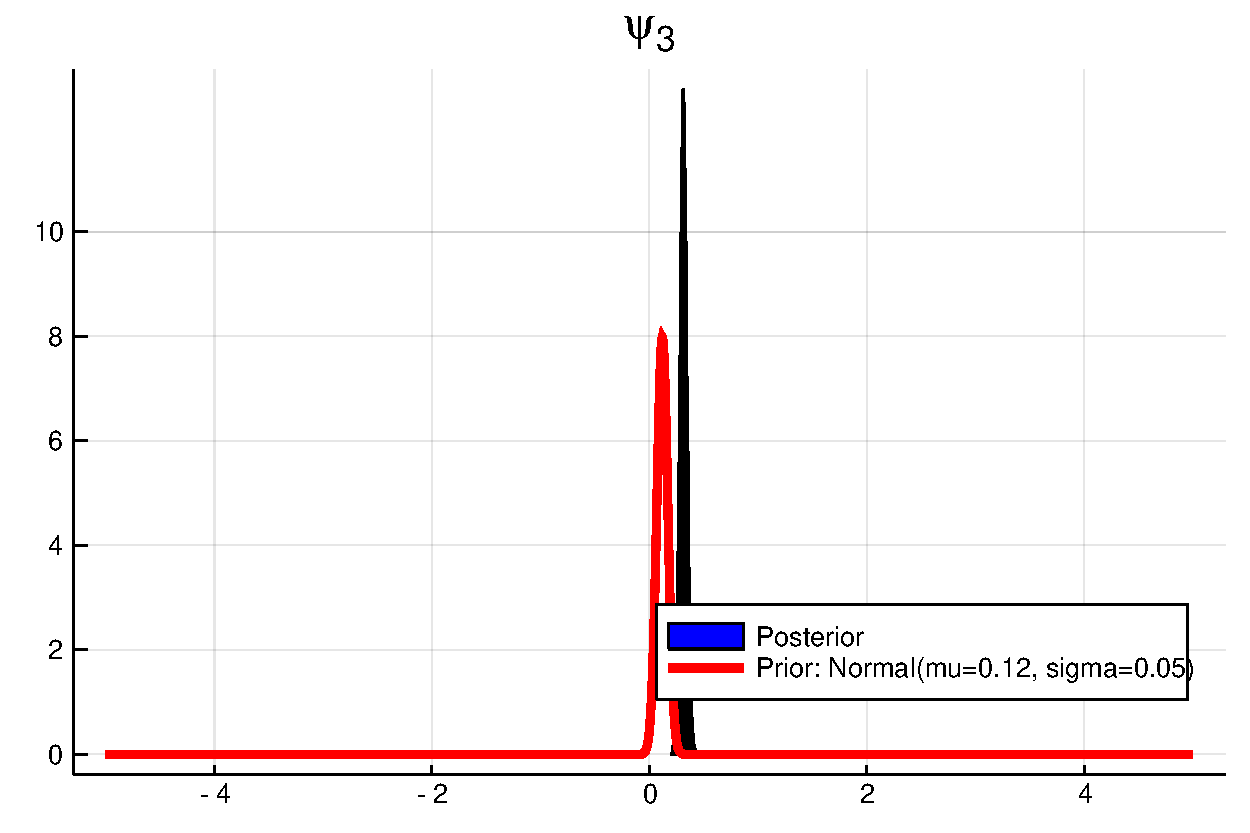
\includegraphics[width=0.45\textwidth]{c:/Mac/Home/Documents/GitHub/rstarBrookings2017/dsge/output_data/m1010/ss20/estimate/figures/prior_posterior_psi3_vint=250826.pdf} &
\includegraphics[width=0.45\textwidth]{c:/Mac/Home/Documents/GitHub/rstarBrookings2017/dsge/output_data/m1010/ss20/estimate/figures/prior_posterior_sigma_c_vint=250826.pdf} \\
\includegraphics[width=0.45\textwidth]{c:/Mac/Home/Documents/GitHub/rstarBrookings2017/dsge/output_data/m1010/ss20/estimate/figures/prior_posterior_rho_vint=250826.pdf} &
\includegraphics[width=0.45\textwidth]{c:/Mac/Home/Documents/GitHub/rstarBrookings2017/dsge/output_data/m1010/ss20/estimate/figures/prior_posterior_spr_vint=250826.pdf} \\
\includegraphics[width=0.45\textwidth]{c:/Mac/Home/Documents/GitHub/rstarBrookings2017/dsge/output_data/m1010/ss20/estimate/figures/prior_posterior_zeta_spb_vint=250826.pdf} &
\includegraphics[width=0.45\textwidth]{c:/Mac/Home/Documents/GitHub/rstarBrookings2017/dsge/output_data/m1010/ss20/estimate/figures/prior_posterior_gamma_vint=250826.pdf} \\
\includegraphics[width=0.45\textwidth]{c:/Mac/Home/Documents/GitHub/rstarBrookings2017/dsge/output_data/m1010/ss20/estimate/figures/prior_posterior_Lmean_vint=250826.pdf} &
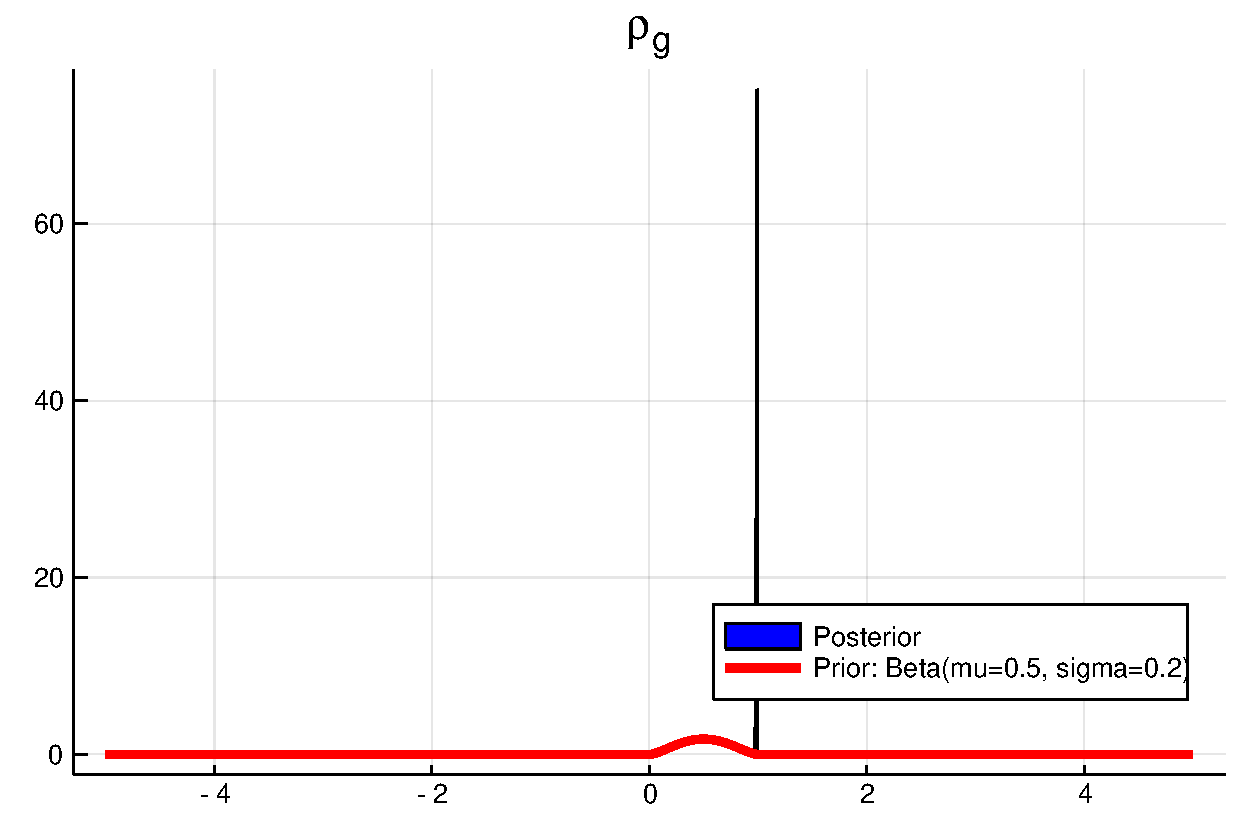
\includegraphics[width=0.45\textwidth]{c:/Mac/Home/Documents/GitHub/rstarBrookings2017/dsge/output_data/m1010/ss20/estimate/figures/prior_posterior_rho_g_vint=250826.pdf} \\
\includegraphics[width=0.45\textwidth]{c:/Mac/Home/Documents/GitHub/rstarBrookings2017/dsge/output_data/m1010/ss20/estimate/figures/prior_posterior_rho_b_liqtil_vint=250826.pdf} &
\includegraphics[width=0.45\textwidth]{c:/Mac/Home/Documents/GitHub/rstarBrookings2017/dsge/output_data/m1010/ss20/estimate/figures/prior_posterior_rho_b_safetil_vint=250826.pdf} \\
\includegraphics[width=0.45\textwidth]{c:/Mac/Home/Documents/GitHub/rstarBrookings2017/dsge/output_data/m1010/ss20/estimate/figures/prior_posterior_rho_mu_vint=250826.pdf} &
\includegraphics[width=0.45\textwidth]{c:/Mac/Home/Documents/GitHub/rstarBrookings2017/dsge/output_data/m1010/ss20/estimate/figures/prior_posterior_rho_z_vint=250826.pdf} \\
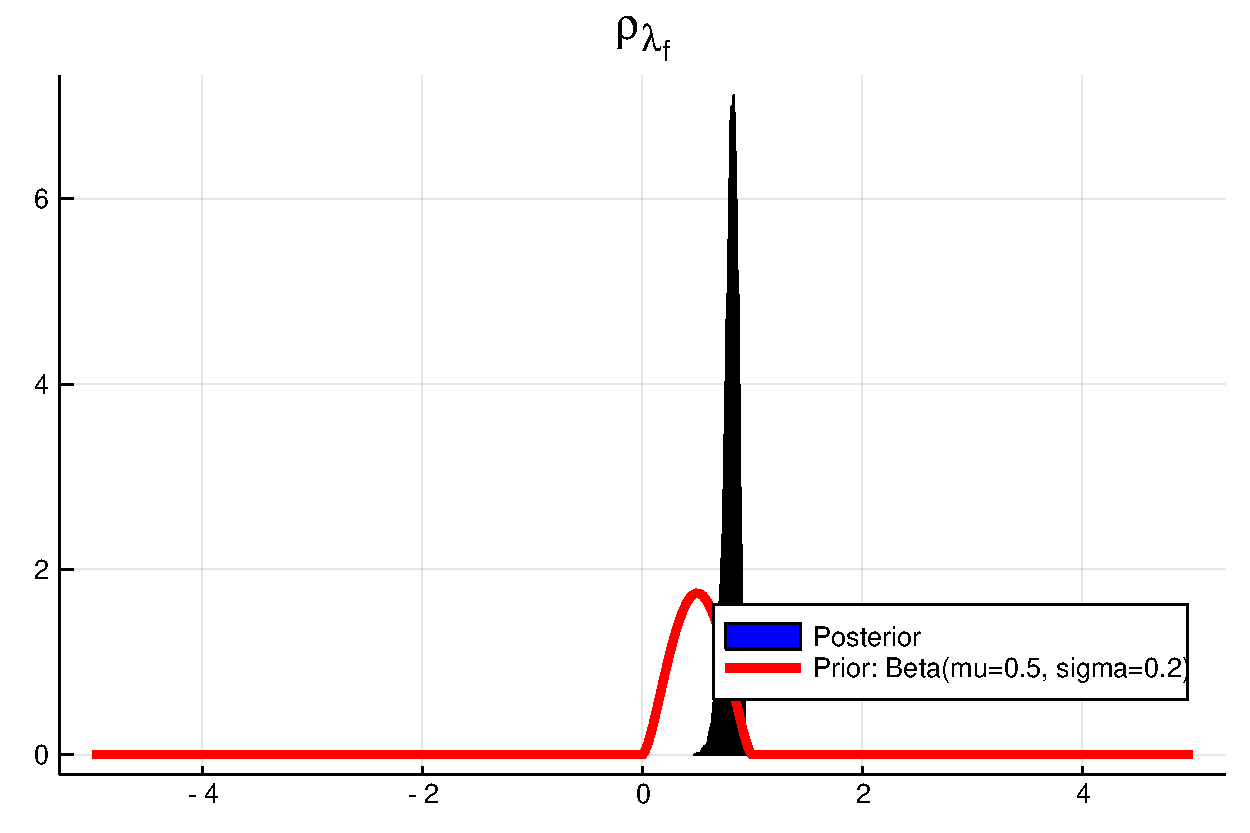
\includegraphics[width=0.45\textwidth]{c:/Mac/Home/Documents/GitHub/rstarBrookings2017/dsge/output_data/m1010/ss20/estimate/figures/prior_posterior_rho_lambda_f_vint=250826.pdf} &
\includegraphics[width=0.45\textwidth]{c:/Mac/Home/Documents/GitHub/rstarBrookings2017/dsge/output_data/m1010/ss20/estimate/figures/prior_posterior_rho_lambda_w_vint=250826.pdf} \\
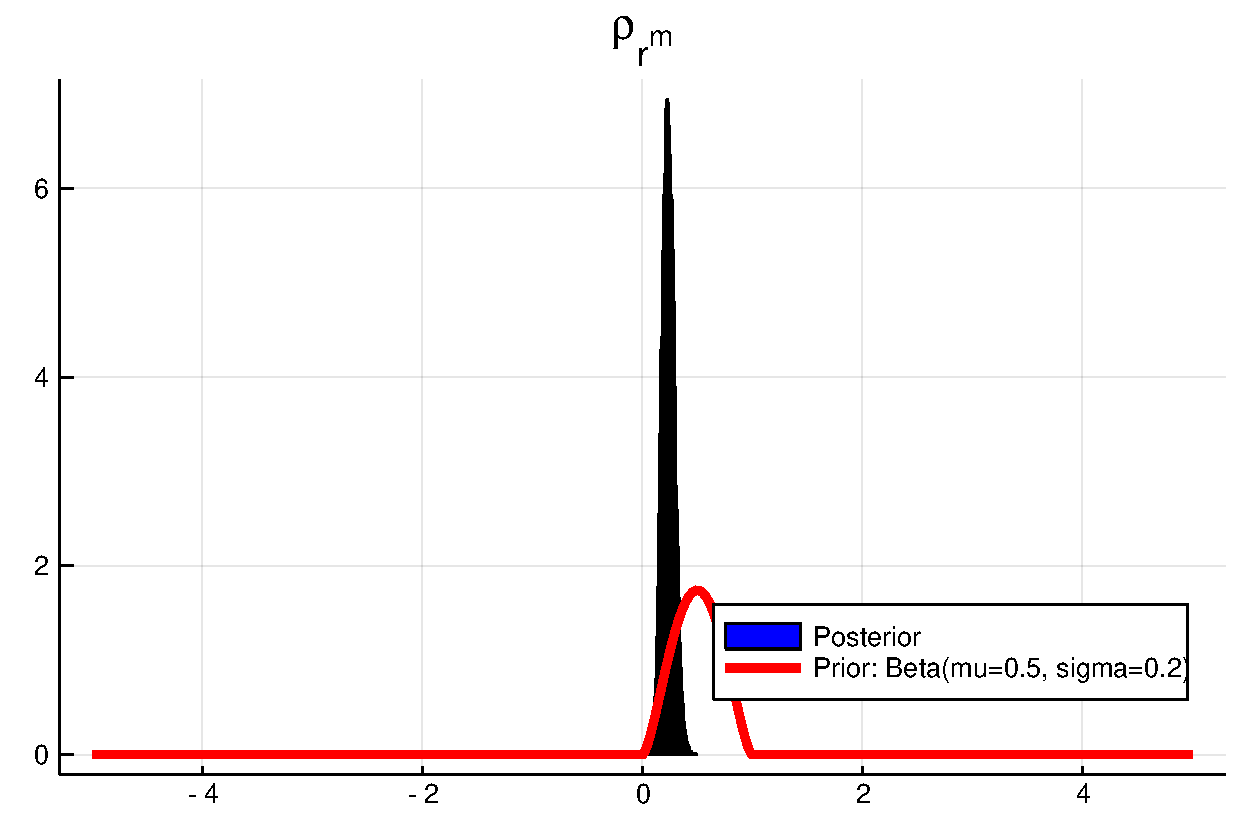
\includegraphics[width=0.45\textwidth]{c:/Mac/Home/Documents/GitHub/rstarBrookings2017/dsge/output_data/m1010/ss20/estimate/figures/prior_posterior_rho_rm_vint=250826.pdf} &
\includegraphics[width=0.45\textwidth]{c:/Mac/Home/Documents/GitHub/rstarBrookings2017/dsge/output_data/m1010/ss20/estimate/figures/prior_posterior_rho_sigma_w_vint=250826.pdf} \\
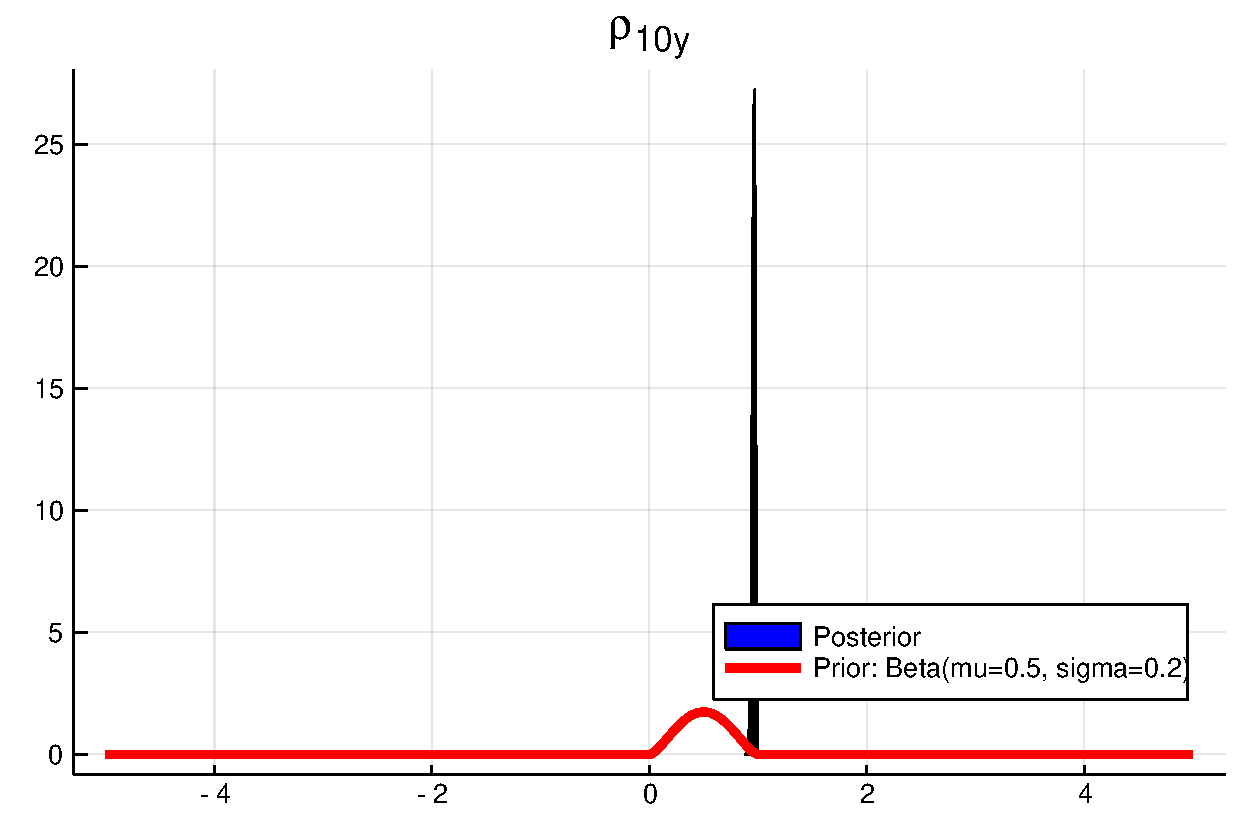
\includegraphics[width=0.45\textwidth]{c:/Mac/Home/Documents/GitHub/rstarBrookings2017/dsge/output_data/m1010/ss20/estimate/figures/prior_posterior_rho_lr_vint=250826.pdf} &
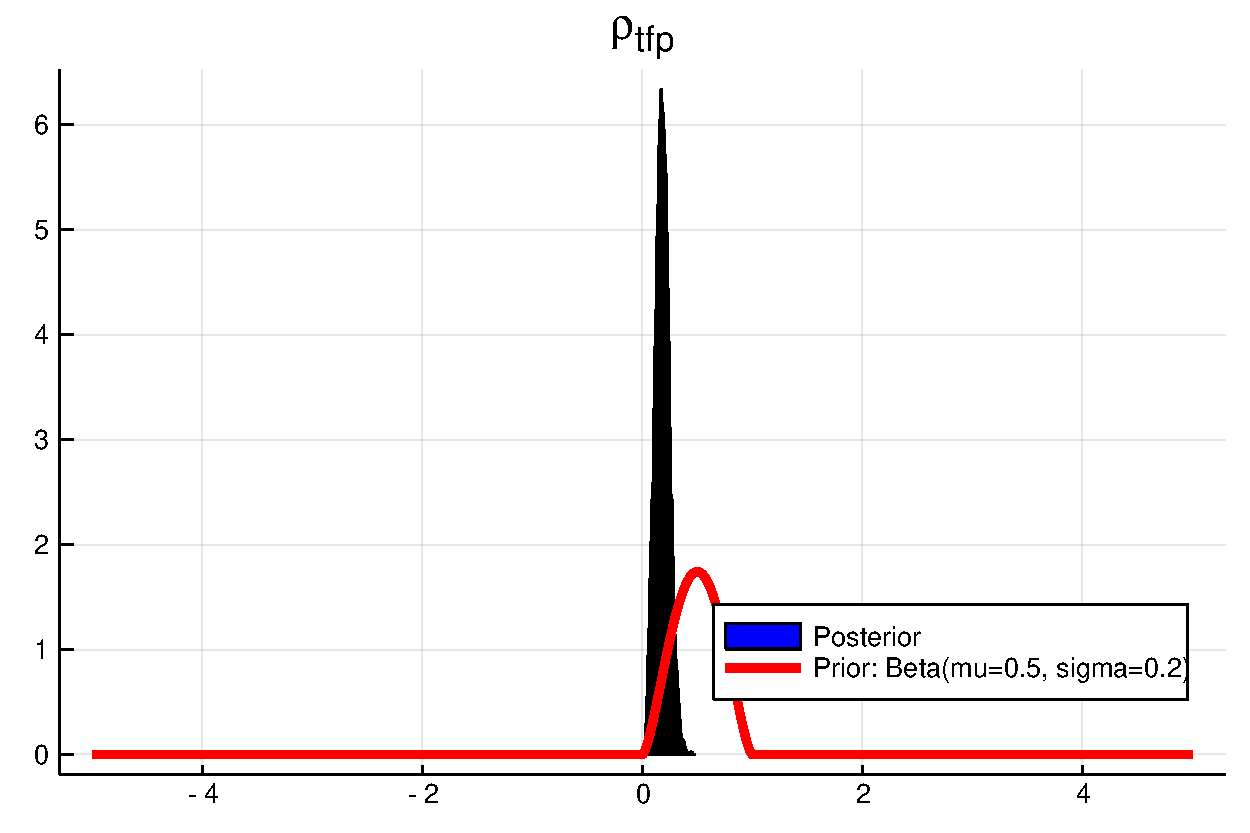
\includegraphics[width=0.45\textwidth]{c:/Mac/Home/Documents/GitHub/rstarBrookings2017/dsge/output_data/m1010/ss20/estimate/figures/prior_posterior_rho_tfp_vint=250826.pdf} \\
\includegraphics[width=0.45\textwidth]{c:/Mac/Home/Documents/GitHub/rstarBrookings2017/dsge/output_data/m1010/ss20/estimate/figures/prior_posterior_rho_gdpdef_vint=250826.pdf} &
\includegraphics[width=0.45\textwidth]{c:/Mac/Home/Documents/GitHub/rstarBrookings2017/dsge/output_data/m1010/ss20/estimate/figures/prior_posterior_rho_corepce_vint=250826.pdf} \\
\includegraphics[width=0.45\textwidth]{c:/Mac/Home/Documents/GitHub/rstarBrookings2017/dsge/output_data/m1010/ss20/estimate/figures/prior_posterior_rho_gdp_vint=250826.pdf} &
\includegraphics[width=0.45\textwidth]{c:/Mac/Home/Documents/GitHub/rstarBrookings2017/dsge/output_data/m1010/ss20/estimate/figures/prior_posterior_rho_gdi_vint=250826.pdf} \\
\includegraphics[width=0.45\textwidth]{c:/Mac/Home/Documents/GitHub/rstarBrookings2017/dsge/output_data/m1010/ss20/estimate/figures/prior_posterior_rho_gdpvar_vint=250826.pdf} &
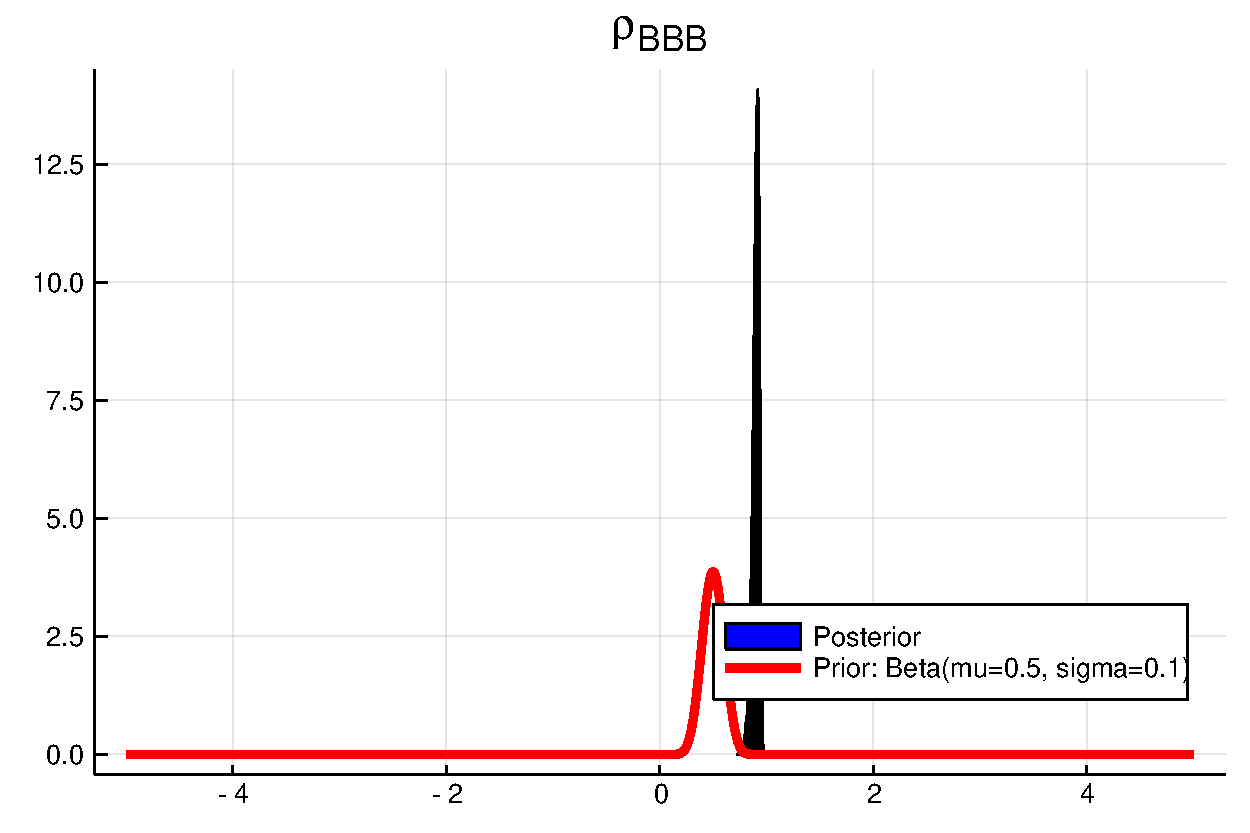
\includegraphics[width=0.45\textwidth]{c:/Mac/Home/Documents/GitHub/rstarBrookings2017/dsge/output_data/m1010/ss20/estimate/figures/prior_posterior_rho_BBB_vint=250826.pdf} \\
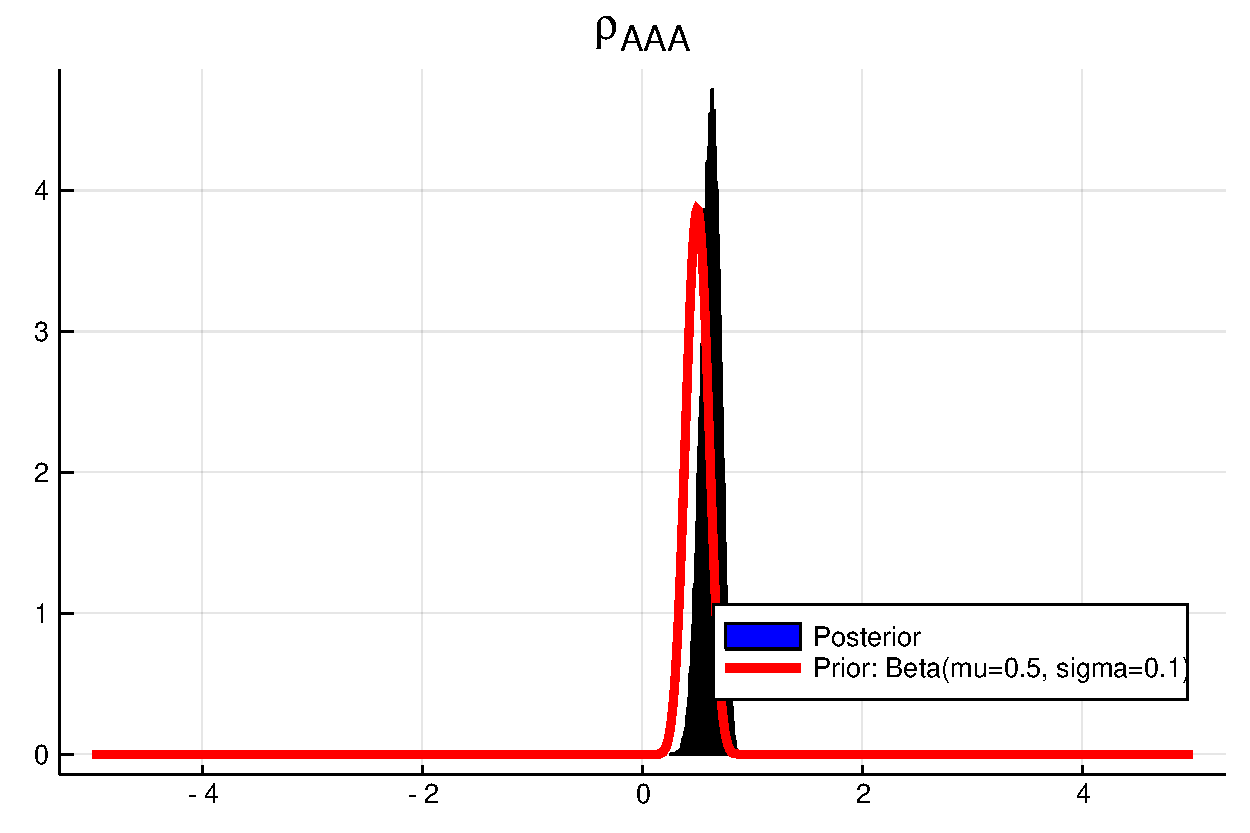
\includegraphics[width=0.45\textwidth]{c:/Mac/Home/Documents/GitHub/rstarBrookings2017/dsge/output_data/m1010/ss20/estimate/figures/prior_posterior_rho_AAA_vint=250826.pdf} &
\includegraphics[width=0.45\textwidth]{c:/Mac/Home/Documents/GitHub/rstarBrookings2017/dsge/output_data/m1010/ss20/estimate/figures/prior_posterior_sigma_g_vint=250826.pdf} \\
\includegraphics[width=0.45\textwidth]{c:/Mac/Home/Documents/GitHub/rstarBrookings2017/dsge/output_data/m1010/ss20/estimate/figures/prior_posterior_sigma_b_liqtil_vint=250826.pdf} &
\includegraphics[width=0.45\textwidth]{c:/Mac/Home/Documents/GitHub/rstarBrookings2017/dsge/output_data/m1010/ss20/estimate/figures/prior_posterior_sigma_b_liqp_vint=250826.pdf} \\
\includegraphics[width=0.45\textwidth]{c:/Mac/Home/Documents/GitHub/rstarBrookings2017/dsge/output_data/m1010/ss20/estimate/figures/prior_posterior_sigma_b_safetil_vint=250826.pdf} &
\includegraphics[width=0.45\textwidth]{c:/Mac/Home/Documents/GitHub/rstarBrookings2017/dsge/output_data/m1010/ss20/estimate/figures/prior_posterior_sigma_b_safep_vint=250826.pdf} \\
\includegraphics[width=0.45\textwidth]{c:/Mac/Home/Documents/GitHub/rstarBrookings2017/dsge/output_data/m1010/ss20/estimate/figures/prior_posterior_sigma_mu_vint=250826.pdf} &
\includegraphics[width=0.45\textwidth]{c:/Mac/Home/Documents/GitHub/rstarBrookings2017/dsge/output_data/m1010/ss20/estimate/figures/prior_posterior_sigma_z_vint=250826.pdf} \\
\includegraphics[width=0.45\textwidth]{c:/Mac/Home/Documents/GitHub/rstarBrookings2017/dsge/output_data/m1010/ss20/estimate/figures/prior_posterior_sigma_lambda_f_vint=250826.pdf} &
\includegraphics[width=0.45\textwidth]{c:/Mac/Home/Documents/GitHub/rstarBrookings2017/dsge/output_data/m1010/ss20/estimate/figures/prior_posterior_sigma_lambda_w_vint=250826.pdf} \\
\includegraphics[width=0.45\textwidth]{c:/Mac/Home/Documents/GitHub/rstarBrookings2017/dsge/output_data/m1010/ss20/estimate/figures/prior_posterior_sigma_r_m_vint=250826.pdf} &
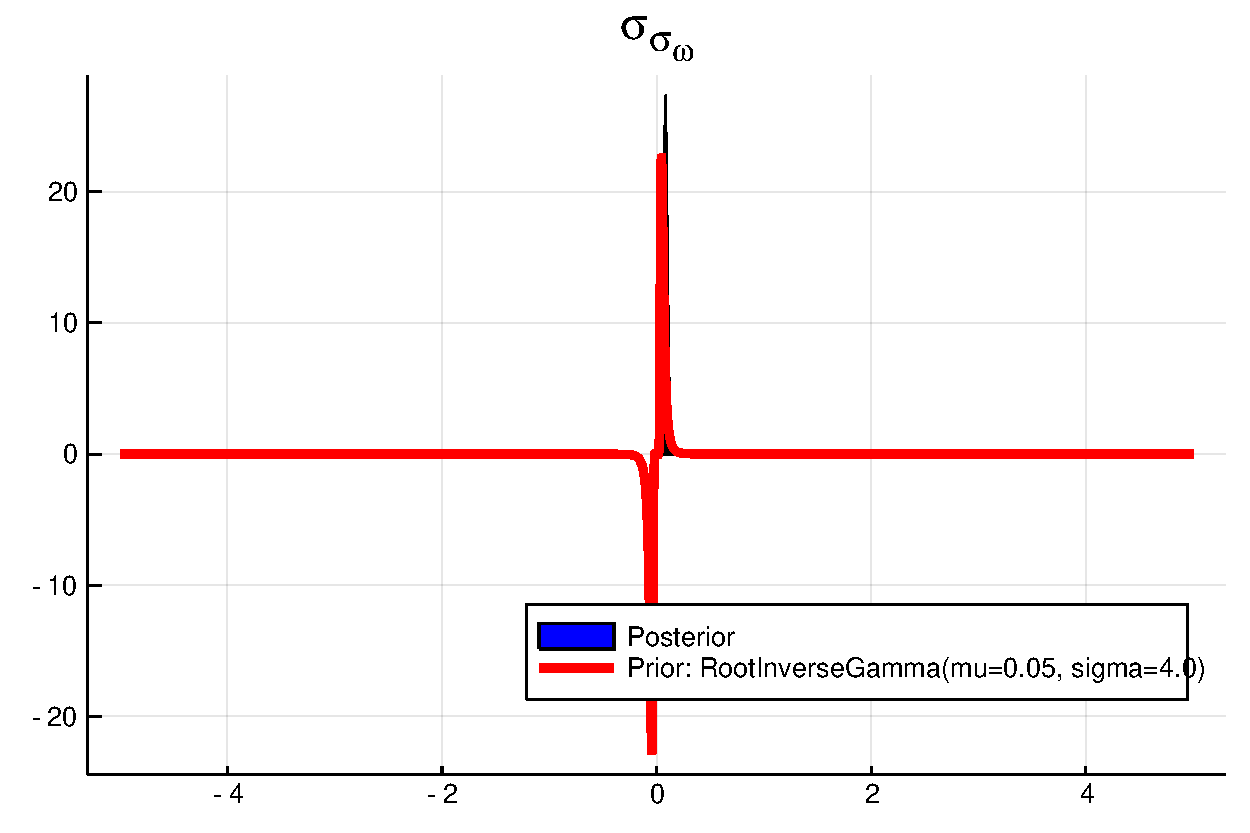
\includegraphics[width=0.45\textwidth]{c:/Mac/Home/Documents/GitHub/rstarBrookings2017/dsge/output_data/m1010/ss20/estimate/figures/prior_posterior_sigma_sigma_omega_vint=250826.pdf} \\
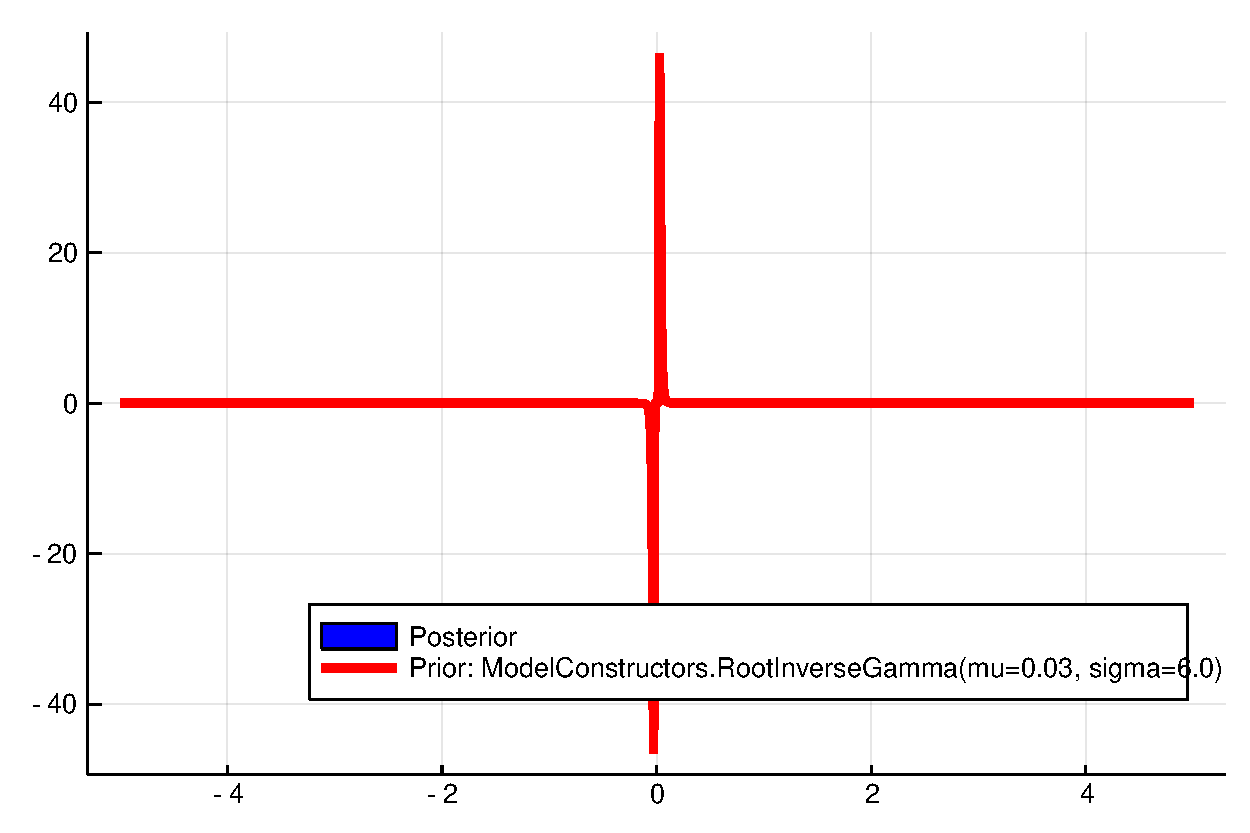
\includegraphics[width=0.45\textwidth]{c:/Mac/Home/Documents/GitHub/rstarBrookings2017/dsge/output_data/m1010/ss20/estimate/figures/prior_posterior_sigma_pi_star_vint=250826.pdf} &
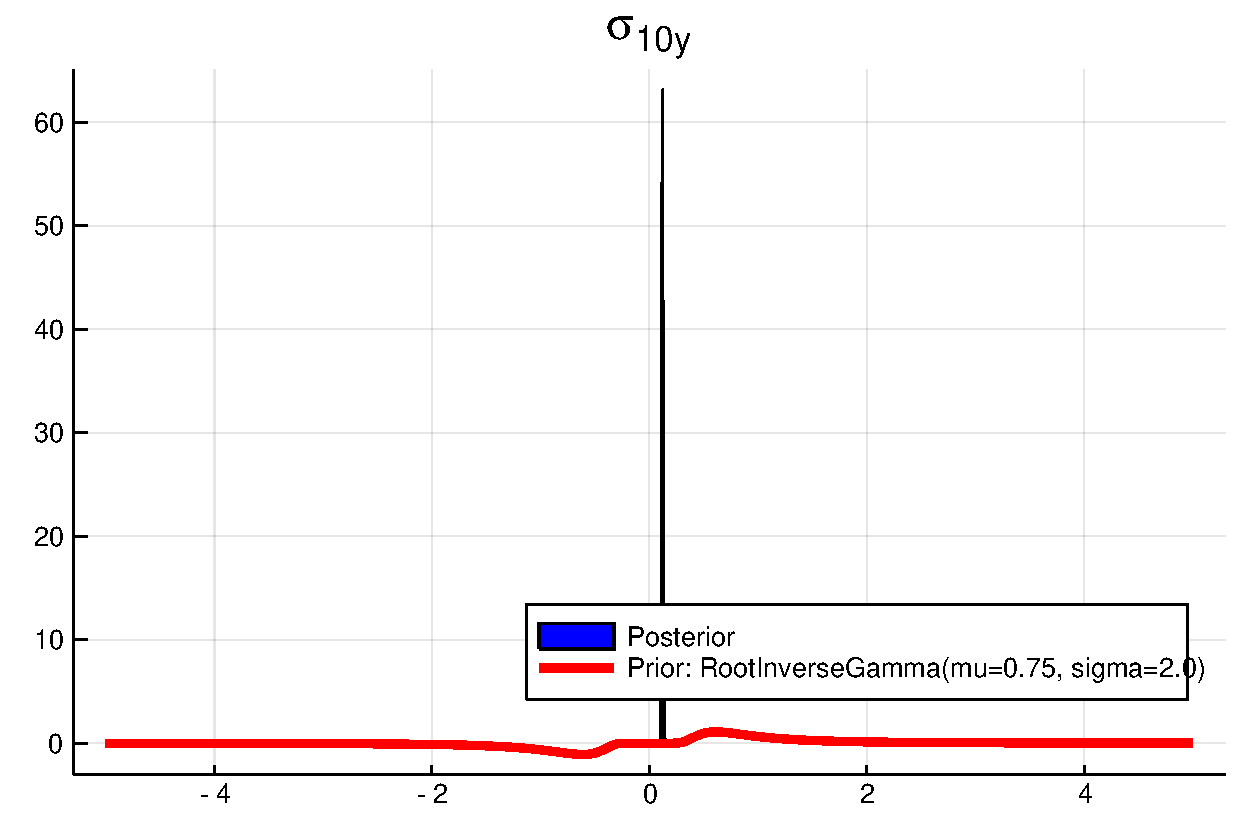
\includegraphics[width=0.45\textwidth]{c:/Mac/Home/Documents/GitHub/rstarBrookings2017/dsge/output_data/m1010/ss20/estimate/figures/prior_posterior_sigma_lr_vint=250826.pdf} \\
\includegraphics[width=0.45\textwidth]{c:/Mac/Home/Documents/GitHub/rstarBrookings2017/dsge/output_data/m1010/ss20/estimate/figures/prior_posterior_sigma_z_p_vint=250826.pdf} &
\includegraphics[width=0.45\textwidth]{c:/Mac/Home/Documents/GitHub/rstarBrookings2017/dsge/output_data/m1010/ss20/estimate/figures/prior_posterior_sigma_tfp_vint=250826.pdf} \\
\includegraphics[width=0.45\textwidth]{c:/Mac/Home/Documents/GitHub/rstarBrookings2017/dsge/output_data/m1010/ss20/estimate/figures/prior_posterior_sigma_gdpdef_vint=250826.pdf} &
\includegraphics[width=0.45\textwidth]{c:/Mac/Home/Documents/GitHub/rstarBrookings2017/dsge/output_data/m1010/ss20/estimate/figures/prior_posterior_sigma_corepce_vint=250826.pdf} \\
\includegraphics[width=0.45\textwidth]{c:/Mac/Home/Documents/GitHub/rstarBrookings2017/dsge/output_data/m1010/ss20/estimate/figures/prior_posterior_sigma_gdp_vint=250826.pdf} &
\includegraphics[width=0.45\textwidth]{c:/Mac/Home/Documents/GitHub/rstarBrookings2017/dsge/output_data/m1010/ss20/estimate/figures/prior_posterior_sigma_gdi_vint=250826.pdf} \\
\includegraphics[width=0.45\textwidth]{c:/Mac/Home/Documents/GitHub/rstarBrookings2017/dsge/output_data/m1010/ss20/estimate/figures/prior_posterior_sigma_BBB_vint=250826.pdf} &
\includegraphics[width=0.45\textwidth]{c:/Mac/Home/Documents/GitHub/rstarBrookings2017/dsge/output_data/m1010/ss20/estimate/figures/prior_posterior_sigma_AAA_vint=250826.pdf} \\
\includegraphics[width=0.45\textwidth]{c:/Mac/Home/Documents/GitHub/rstarBrookings2017/dsge/output_data/m1010/ss20/estimate/figures/prior_posterior_sigma_r_m1_vint=250826.pdf} &
\includegraphics[width=0.45\textwidth]{c:/Mac/Home/Documents/GitHub/rstarBrookings2017/dsge/output_data/m1010/ss20/estimate/figures/prior_posterior_sigma_r_m2_vint=250826.pdf} \\
\includegraphics[width=0.45\textwidth]{c:/Mac/Home/Documents/GitHub/rstarBrookings2017/dsge/output_data/m1010/ss20/estimate/figures/prior_posterior_sigma_r_m3_vint=250826.pdf} &
\includegraphics[width=0.45\textwidth]{c:/Mac/Home/Documents/GitHub/rstarBrookings2017/dsge/output_data/m1010/ss20/estimate/figures/prior_posterior_sigma_r_m4_vint=250826.pdf} \\
\includegraphics[width=0.45\textwidth]{c:/Mac/Home/Documents/GitHub/rstarBrookings2017/dsge/output_data/m1010/ss20/estimate/figures/prior_posterior_sigma_r_m5_vint=250826.pdf} &
\includegraphics[width=0.45\textwidth]{c:/Mac/Home/Documents/GitHub/rstarBrookings2017/dsge/output_data/m1010/ss20/estimate/figures/prior_posterior_sigma_r_m6_vint=250826.pdf} \\
\includegraphics[width=0.45\textwidth]{c:/Mac/Home/Documents/GitHub/rstarBrookings2017/dsge/output_data/m1010/ss20/estimate/figures/prior_posterior_sigma_r_m7_vint=250826.pdf} &
\includegraphics[width=0.45\textwidth]{c:/Mac/Home/Documents/GitHub/rstarBrookings2017/dsge/output_data/m1010/ss20/estimate/figures/prior_posterior_sigma_r_m8_vint=250826.pdf} \\
\includegraphics[width=0.45\textwidth]{c:/Mac/Home/Documents/GitHub/rstarBrookings2017/dsge/output_data/m1010/ss20/estimate/figures/prior_posterior_sigma_r_m9_vint=250826.pdf} &
\includegraphics[width=0.45\textwidth]{c:/Mac/Home/Documents/GitHub/rstarBrookings2017/dsge/output_data/m1010/ss20/estimate/figures/prior_posterior_sigma_r_m10_vint=250826.pdf} \\
\includegraphics[width=0.45\textwidth]{c:/Mac/Home/Documents/GitHub/rstarBrookings2017/dsge/output_data/m1010/ss20/estimate/figures/prior_posterior_sigma_r_m11_vint=250826.pdf} &
\includegraphics[width=0.45\textwidth]{c:/Mac/Home/Documents/GitHub/rstarBrookings2017/dsge/output_data/m1010/ss20/estimate/figures/prior_posterior_sigma_r_m12_vint=250826.pdf} \\
\includegraphics[width=0.45\textwidth]{c:/Mac/Home/Documents/GitHub/rstarBrookings2017/dsge/output_data/m1010/ss20/estimate/figures/prior_posterior_eta_gz_vint=250826.pdf} &
\includegraphics[width=0.45\textwidth]{c:/Mac/Home/Documents/GitHub/rstarBrookings2017/dsge/output_data/m1010/ss20/estimate/figures/prior_posterior_eta_lambda_f_vint=250826.pdf} \\
\includegraphics[width=0.45\textwidth]{c:/Mac/Home/Documents/GitHub/rstarBrookings2017/dsge/output_data/m1010/ss20/estimate/figures/prior_posterior_eta_lambda_w_vint=250826.pdf} &
\includegraphics[width=0.45\textwidth]{c:/Mac/Home/Documents/GitHub/rstarBrookings2017/dsge/output_data/m1010/ss20/estimate/figures/prior_posterior_Gamma_gdpdef_vint=250826.pdf} \\
\includegraphics[width=0.45\textwidth]{c:/Mac/Home/Documents/GitHub/rstarBrookings2017/dsge/output_data/m1010/ss20/estimate/figures/prior_posterior_delta_gdpdef_vint=250826.pdf} &
\end{longtable}

\clearpage
\subsection{Moments}

\input{c:/Mac/Home/Documents/GitHub/rstarBrookings2017/dsge/output_data/m1010/ss20/estimate/tables/moments_vint=250826.tex}


\clearpage
\section{Forecast}

\subsection{Specification}

\begin{itemize}
  \item Forecast type: mode
  \item Forecast conditional type: none
  \item Estimation used: \path{c:/Mac/Home/Documents/GitHub/rstarBrookings2017/dsge/output_data/m1010/ss20/estimate/raw/paramsmode_vint=250826.h5}
\end{itemize}
\clearpage
\subsection{Forecasts}

\subsubsection{Observables}
\begin{longtable}{c}
\includegraphics[height=0.4\textheight]{c:/Mac/Home/Documents/GitHub/rstarBrookings2017/dsge/output_data/m1010/ss20/forecast/figures/forecast_obs_gdp_cond=none_para=mode_vint=250826.pdf} \\
\includegraphics[height=0.4\textheight]{c:/Mac/Home/Documents/GitHub/rstarBrookings2017/dsge/output_data/m1010/ss20/forecast/figures/forecast_obs_hours_cond=none_para=mode_vint=250826.pdf} \\
\includegraphics[height=0.4\textheight]{c:/Mac/Home/Documents/GitHub/rstarBrookings2017/dsge/output_data/m1010/ss20/forecast/figures/forecast_obs_wages_cond=none_para=mode_vint=250826.pdf} \\
\includegraphics[height=0.4\textheight]{c:/Mac/Home/Documents/GitHub/rstarBrookings2017/dsge/output_data/m1010/ss20/forecast/figures/forecast_obs_gdpdeflator_cond=none_para=mode_vint=250826.pdf} \\
\includegraphics[height=0.4\textheight]{c:/Mac/Home/Documents/GitHub/rstarBrookings2017/dsge/output_data/m1010/ss20/forecast/figures/forecast_obs_corepce_cond=none_para=mode_vint=250826.pdf} \\
\includegraphics[height=0.4\textheight]{c:/Mac/Home/Documents/GitHub/rstarBrookings2017/dsge/output_data/m1010/ss20/forecast/figures/forecast_obs_nominalrate_cond=none_para=mode_vint=250826.pdf} \\
\includegraphics[height=0.4\textheight]{c:/Mac/Home/Documents/GitHub/rstarBrookings2017/dsge/output_data/m1010/ss20/forecast/figures/forecast_obs_consumption_cond=none_para=mode_vint=250826.pdf} \\
\includegraphics[height=0.4\textheight]{c:/Mac/Home/Documents/GitHub/rstarBrookings2017/dsge/output_data/m1010/ss20/forecast/figures/forecast_obs_investment_cond=none_para=mode_vint=250826.pdf} \\
\includegraphics[height=0.4\textheight]{c:/Mac/Home/Documents/GitHub/rstarBrookings2017/dsge/output_data/m1010/ss20/forecast/figures/forecast_obs_BBBspread_cond=none_para=mode_vint=250826.pdf} \\
\includegraphics[height=0.4\textheight]{c:/Mac/Home/Documents/GitHub/rstarBrookings2017/dsge/output_data/m1010/ss20/forecast/figures/forecast_obs_longinflation_cond=none_para=mode_vint=250826.pdf} \\
\includegraphics[height=0.4\textheight]{c:/Mac/Home/Documents/GitHub/rstarBrookings2017/dsge/output_data/m1010/ss20/forecast/figures/forecast_obs_longrate_cond=none_para=mode_vint=250826.pdf} \\
\includegraphics[height=0.4\textheight]{c:/Mac/Home/Documents/GitHub/rstarBrookings2017/dsge/output_data/m1010/ss20/forecast/figures/forecast_obs_tfp_cond=none_para=mode_vint=250826.pdf} \\
\includegraphics[height=0.4\textheight]{c:/Mac/Home/Documents/GitHub/rstarBrookings2017/dsge/output_data/m1010/ss20/forecast/figures/forecast_obs_gdi_cond=none_para=mode_vint=250826.pdf} \\
\includegraphics[height=0.4\textheight]{c:/Mac/Home/Documents/GitHub/rstarBrookings2017/dsge/output_data/m1010/ss20/forecast/figures/forecast_obs_AAAspread_cond=none_para=mode_vint=250826.pdf} \\
\includegraphics[height=0.4\textheight]{c:/Mac/Home/Documents/GitHub/rstarBrookings2017/dsge/output_data/m1010/ss20/forecast/figures/forecast_obs_nominalrate1_cond=none_para=mode_vint=250826.pdf} \\
\includegraphics[height=0.4\textheight]{c:/Mac/Home/Documents/GitHub/rstarBrookings2017/dsge/output_data/m1010/ss20/forecast/figures/forecast_obs_nominalrate2_cond=none_para=mode_vint=250826.pdf} \\
\includegraphics[height=0.4\textheight]{c:/Mac/Home/Documents/GitHub/rstarBrookings2017/dsge/output_data/m1010/ss20/forecast/figures/forecast_obs_nominalrate3_cond=none_para=mode_vint=250826.pdf} \\
\includegraphics[height=0.4\textheight]{c:/Mac/Home/Documents/GitHub/rstarBrookings2017/dsge/output_data/m1010/ss20/forecast/figures/forecast_obs_nominalrate4_cond=none_para=mode_vint=250826.pdf} \\
\includegraphics[height=0.4\textheight]{c:/Mac/Home/Documents/GitHub/rstarBrookings2017/dsge/output_data/m1010/ss20/forecast/figures/forecast_obs_nominalrate5_cond=none_para=mode_vint=250826.pdf} \\
\includegraphics[height=0.4\textheight]{c:/Mac/Home/Documents/GitHub/rstarBrookings2017/dsge/output_data/m1010/ss20/forecast/figures/forecast_obs_nominalrate6_cond=none_para=mode_vint=250826.pdf} \\
\end{longtable}


\subsubsection{Pseudo-Observables}
\begin{longtable}{c}
\includegraphics[height=0.4\textheight]{c:/Mac/Home/Documents/GitHub/rstarBrookings2017/dsge/output_data/m1010/ss20/forecast/figures/forecast_y_t_cond=none_para=mode_vint=250826.pdf} \\
\includegraphics[height=0.4\textheight]{c:/Mac/Home/Documents/GitHub/rstarBrookings2017/dsge/output_data/m1010/ss20/forecast/figures/forecast_y_f_t_cond=none_para=mode_vint=250826.pdf} \\
\includegraphics[height=0.4\textheight]{c:/Mac/Home/Documents/GitHub/rstarBrookings2017/dsge/output_data/m1010/ss20/forecast/figures/forecast_OutputGap_cond=none_para=mode_vint=250826.pdf} \\
\includegraphics[height=0.4\textheight]{c:/Mac/Home/Documents/GitHub/rstarBrookings2017/dsge/output_data/m1010/ss20/forecast/figures/forecast_Hours_cond=none_para=mode_vint=250826.pdf} \\
\includegraphics[height=0.4\textheight]{c:/Mac/Home/Documents/GitHub/rstarBrookings2017/dsge/output_data/m1010/ss20/forecast/figures/forecast_RealNaturalRate_cond=none_para=mode_vint=250826.pdf} \\
\includegraphics[height=0.4\textheight]{c:/Mac/Home/Documents/GitHub/rstarBrookings2017/dsge/output_data/m1010/ss20/forecast/figures/forecast_ExAnteRealRate_cond=none_para=mode_vint=250826.pdf} \\
\includegraphics[height=0.4\textheight]{c:/Mac/Home/Documents/GitHub/rstarBrookings2017/dsge/output_data/m1010/ss20/forecast/figures/forecast_NominalNaturalRate_cond=none_para=mode_vint=250826.pdf} \\
\includegraphics[height=0.4\textheight]{c:/Mac/Home/Documents/GitHub/rstarBrookings2017/dsge/output_data/m1010/ss20/forecast/figures/forecast_NominalFFR_cond=none_para=mode_vint=250826.pdf} \\
\includegraphics[height=0.4\textheight]{c:/Mac/Home/Documents/GitHub/rstarBrookings2017/dsge/output_data/m1010/ss20/forecast/figures/forecast_ExpectedAvg5YearRealRate_cond=none_para=mode_vint=250826.pdf} \\
\includegraphics[height=0.4\textheight]{c:/Mac/Home/Documents/GitHub/rstarBrookings2017/dsge/output_data/m1010/ss20/forecast/figures/forecast_ExpectedAvg5YearRealNaturalRate_cond=none_para=mode_vint=250826.pdf} \\
\includegraphics[height=0.4\textheight]{c:/Mac/Home/Documents/GitHub/rstarBrookings2017/dsge/output_data/m1010/ss20/forecast/figures/forecast_ExpectedAvg10YearRealRate_cond=none_para=mode_vint=250826.pdf} \\
\includegraphics[height=0.4\textheight]{c:/Mac/Home/Documents/GitHub/rstarBrookings2017/dsge/output_data/m1010/ss20/forecast/figures/forecast_ExpectedAvg10YearRealNaturalRate_cond=none_para=mode_vint=250826.pdf} \\
\includegraphics[height=0.4\textheight]{c:/Mac/Home/Documents/GitHub/rstarBrookings2017/dsge/output_data/m1010/ss20/forecast/figures/forecast_ExpectedAvg20YearRealRate_cond=none_para=mode_vint=250826.pdf} \\
\includegraphics[height=0.4\textheight]{c:/Mac/Home/Documents/GitHub/rstarBrookings2017/dsge/output_data/m1010/ss20/forecast/figures/forecast_ExpectedAvg20YearRealNaturalRate_cond=none_para=mode_vint=250826.pdf} \\
\includegraphics[height=0.4\textheight]{c:/Mac/Home/Documents/GitHub/rstarBrookings2017/dsge/output_data/m1010/ss20/forecast/figures/forecast_Forward5YearRealRate_cond=none_para=mode_vint=250826.pdf} \\
\includegraphics[height=0.4\textheight]{c:/Mac/Home/Documents/GitHub/rstarBrookings2017/dsge/output_data/m1010/ss20/forecast/figures/forecast_Forward5YearRealNaturalRate_cond=none_para=mode_vint=250826.pdf} \\
\includegraphics[height=0.4\textheight]{c:/Mac/Home/Documents/GitHub/rstarBrookings2017/dsge/output_data/m1010/ss20/forecast/figures/forecast_Forward10YearRealRate_cond=none_para=mode_vint=250826.pdf} \\
\includegraphics[height=0.4\textheight]{c:/Mac/Home/Documents/GitHub/rstarBrookings2017/dsge/output_data/m1010/ss20/forecast/figures/forecast_Forward10YearRealNaturalRate_cond=none_para=mode_vint=250826.pdf} \\
\includegraphics[height=0.4\textheight]{c:/Mac/Home/Documents/GitHub/rstarBrookings2017/dsge/output_data/m1010/ss20/forecast/figures/forecast_Forward20YearRealRate_cond=none_para=mode_vint=250826.pdf} \\
\includegraphics[height=0.4\textheight]{c:/Mac/Home/Documents/GitHub/rstarBrookings2017/dsge/output_data/m1010/ss20/forecast/figures/forecast_Forward20YearRealNaturalRate_cond=none_para=mode_vint=250826.pdf} \\
\includegraphics[height=0.4\textheight]{c:/Mac/Home/Documents/GitHub/rstarBrookings2017/dsge/output_data/m1010/ss20/forecast/figures/forecast_Forward30YearRealRate_cond=none_para=mode_vint=250826.pdf} \\
\includegraphics[height=0.4\textheight]{c:/Mac/Home/Documents/GitHub/rstarBrookings2017/dsge/output_data/m1010/ss20/forecast/figures/forecast_Forward30YearRealNaturalRate_cond=none_para=mode_vint=250826.pdf} \\
\end{longtable}

\clearpage
\subsection{Mean Forecast Estimates}
\begin{table}[h!]
\centering
\begin{tabular}{l | c | c | c | c }
& 2025 & 2026 & 2027 & 2028 \\
\hline
\hline
